\section{Мета}
Отримання практичних навичок встановлення та
налаштування віртуальних машин.


\section{Завдання}
Визначити тип відеоконтролера, його режим та дату створення BIOS;
перевірити справність НМД


\section{Хід роботи}
\subsection{Код програми}
\lstinputlisting[language=Rust, style=colouredRust]{\codeDirectory/lab2/main.c}

\subsection{Результат роботи програми}
\begin{figure}[ht!]
    \centering
    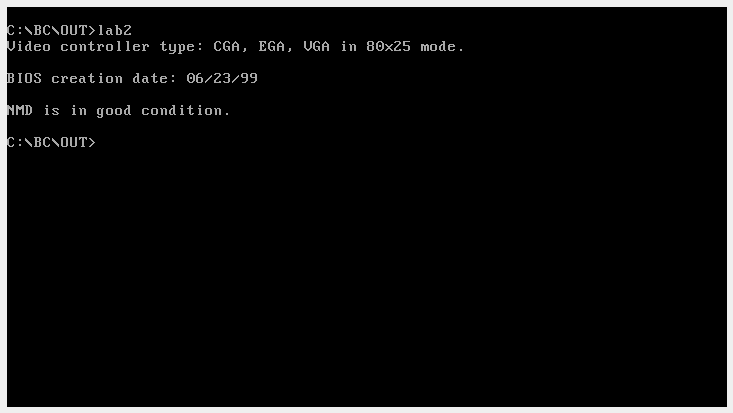
\includegraphics[width=0.9\textwidth]{\assetsDirectory/res.png}
    \caption{Результат роботи програми}
\end{figure}

\clearpage
\section{Висновки}
В ході виконання практичної роботи було отримано навички роботи з
низькорівневим доступом до системної пам'яті та аналізу конфігураційних параметрів комп'ютерної системи.
Було створено програму на мові \textbf{C}, яка зчитує слово конфігурації BIOS за адресою \texttt{0040:0010h}
і визначає тип та режим відеоконтролера, дату створення BIOS та справність НМД.
